\documentclass[fleqn]{beamer}

%\usepackage[spanish]{babel}
\usepackage[font=scriptsize]{caption}
\usepackage{amsmath,amssymb}
\usepackage{graphicx}
\usepackage{subfig}
\usepackage{booktabs}
\usepackage{multirow}

\setbeamerfont{bibliography item}{size=\footnotesize}
\setbeamerfont{bibliography entry author}{size=\footnotesize}
\setbeamerfont{bibliography entry title}{size=\footnotesize}
\setbeamerfont{bibliography entry location}{size=\footnotesize}
\setbeamerfont{bibliography entry note}{size=\footnotesize}


%

% vertical separator macro
\newcommand{\vsep}{
  \column{0.0\textwidth}
    \begin{tikzpicture}
      \draw[very thick,black!10] (0,0) -- (0,7.3);
    \end{tikzpicture}
}

% More space between lines in align
\setlength{\mathindent}{0pt}

% Beamer theme
\usetheme{ZMBZFMK}
\usefonttheme[onlysmall]{structurebold}
\mode<presentation>
%\setbeamercovered{transparent=10}

% align spacing
\setlength{\jot}{0pt}


\AtBeginSection[]
{
  \begin{frame}
    \frametitle{Table of Contents}
    \tableofcontents[currentsection]
  \end{frame}
}
\AtBeginSubsection[]
{
  \begin{frame}
    \frametitle{Table of Contents}
    \tableofcontents[currentsubsection]
  \end{frame}
}
%\usepackage[backend=biber,style=numeric, citestyle=ieee]{biblatex}
%\addbibresource{main.bib}

%\bibliography{references}
% Only the First Slide
\title{CNUH Latex Template}
\subtitle{Latex template for CNU student's presentation}
\author{Nguyen Trong Nghia}
\institute[Chonnam National University]{ Adviser:}
%\date{October 26, 2022} %\today


% Portada
\begin{document}
\begin{frame}
  \titlepage
\end{frame}


% Frame 1

\section{Section 1}
\begin{frame}{Frame 1 of section 1}
    \begin{itemize}
        \item Sample reference \cite{Davis}
    \end{itemize}
\end{frame}
    
\begin{frame}{Frame 2 of section 1}
    \begin{figure}
        \centering
        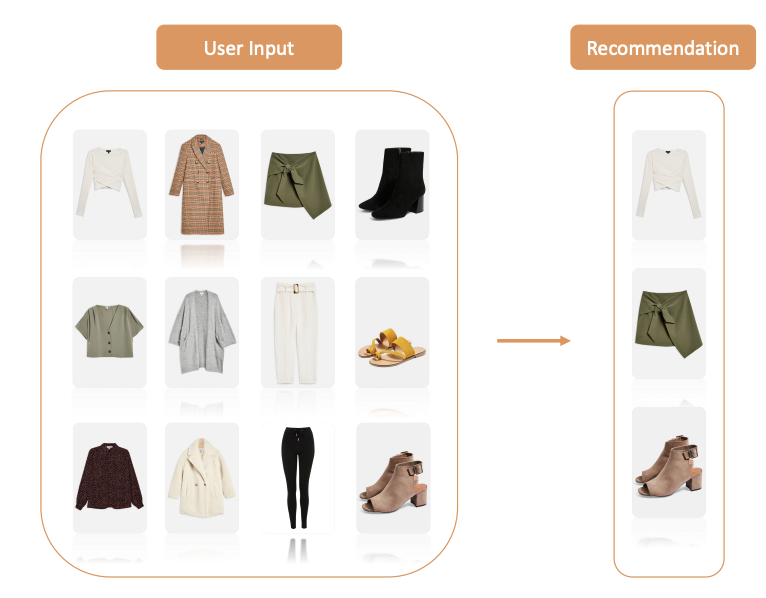
\includegraphics[width=0.6\textwidth]{img/Fashion_sys.png}
        \caption{Sample figure}
        \label{fig:my_label}
    \end{figure}
\end{frame}

\section{Section 2}
\begin{frame}{Frame 1 of section 2}
    % Please add the following required packages to your document preamble:
    % \usepackage{booktabs}
    \begin{table}[]
    \begin{tabular}{@{}lll@{}}
    \toprule
    Model    & F1-score & AUC   \\ \midrule
    Bi-LSTM  & 0.651    & 0.665 \\
    Proposed & 0.723    & 0.751 \\ \bottomrule
    \end{tabular}
    \caption{Sample table}
    \end{table}
\end{frame}

\begin{frame}
        \frametitle{References}
        \bibliographystyle{IEEEtran}
        \bibliography{main.bib}
\end{frame}
\begin{frame}[plain,noframenumbering]{}
  \centering \Large
  \emph{Thank you!}
\end{frame}

\end{document}